\section[Prevention]{Prevention}

To prevent malware infiltration, both the Windows development team and
Anti-Virus vendors have tried to apply new technology to secure the operating
system. Here we list some advancement that has helped minimize the spread of
malware.

\subsection[Signature enforcement]{Signature enforcement}

In the past, drivers can be loaded on the system with only an admin privilege.
It was a bad practice, any driver, trusted or untrusted, can be loaded inside
Windows. Windows then forces driver creators/distributors to sign their drivers
using a Windows certificate to prevent untrusted drivers. Signing the driver
costs money and includes a code review that would prevent a malicious driver
created.

However, some malware writers are brilliant, they could reuse a legitimate
driver with vulnerability and \textit{exploit} the driver to make it work as
they wanted. The driver is trusted, but the bug inside the driver is used as an
attack vector. An example is RobinHood (2020) malware reused the
\texttt{GDRV.SYS} driver from Gigabyte \cite{robinhood}.

\subsection[Patchguard]{Patchguard}

Windows prevents malware from modifying kernel components with Patchguard.  In
the past, malware used to \textit{patch}, modify, some kernel components to
gain control of the system.  It was prevented after Windows introduced
Patchguard, a way to detect edits in the kernel code and crash the system when
editing detected.

Although this was a good approach, Windows still has some failure. The report
on malware bypassing Patchguard is GhostHook (2017) \cite{ghosthook}, and two
research to bypass the Patchguard are InfinityHook (2019) \cite{infinityhook},
and ByePg (2019) \cite{byepg}.

\subsection[On-access scanning]{On-access scanning}

On-access scanning is a technique developed by Anti-Virus vendors to scan the
file for malware evidence on accessing the file. They installed a hook in the
Windows API for file access, and scan the file on any read/write access. If the
file matches a previously defined signature, the Anti-Virus will prevent access
and warn the user for removal. The algorithm is illustrated in Figure
\ref{fig:onaccessscan}, this algorithm is used by McAfee Anti-Virus
\cite{onaccessscan}.

\begin{figure}[h]
  \centering
  \caption{McAffee On-access scanning}
  \label{fig:onaccessscan}
  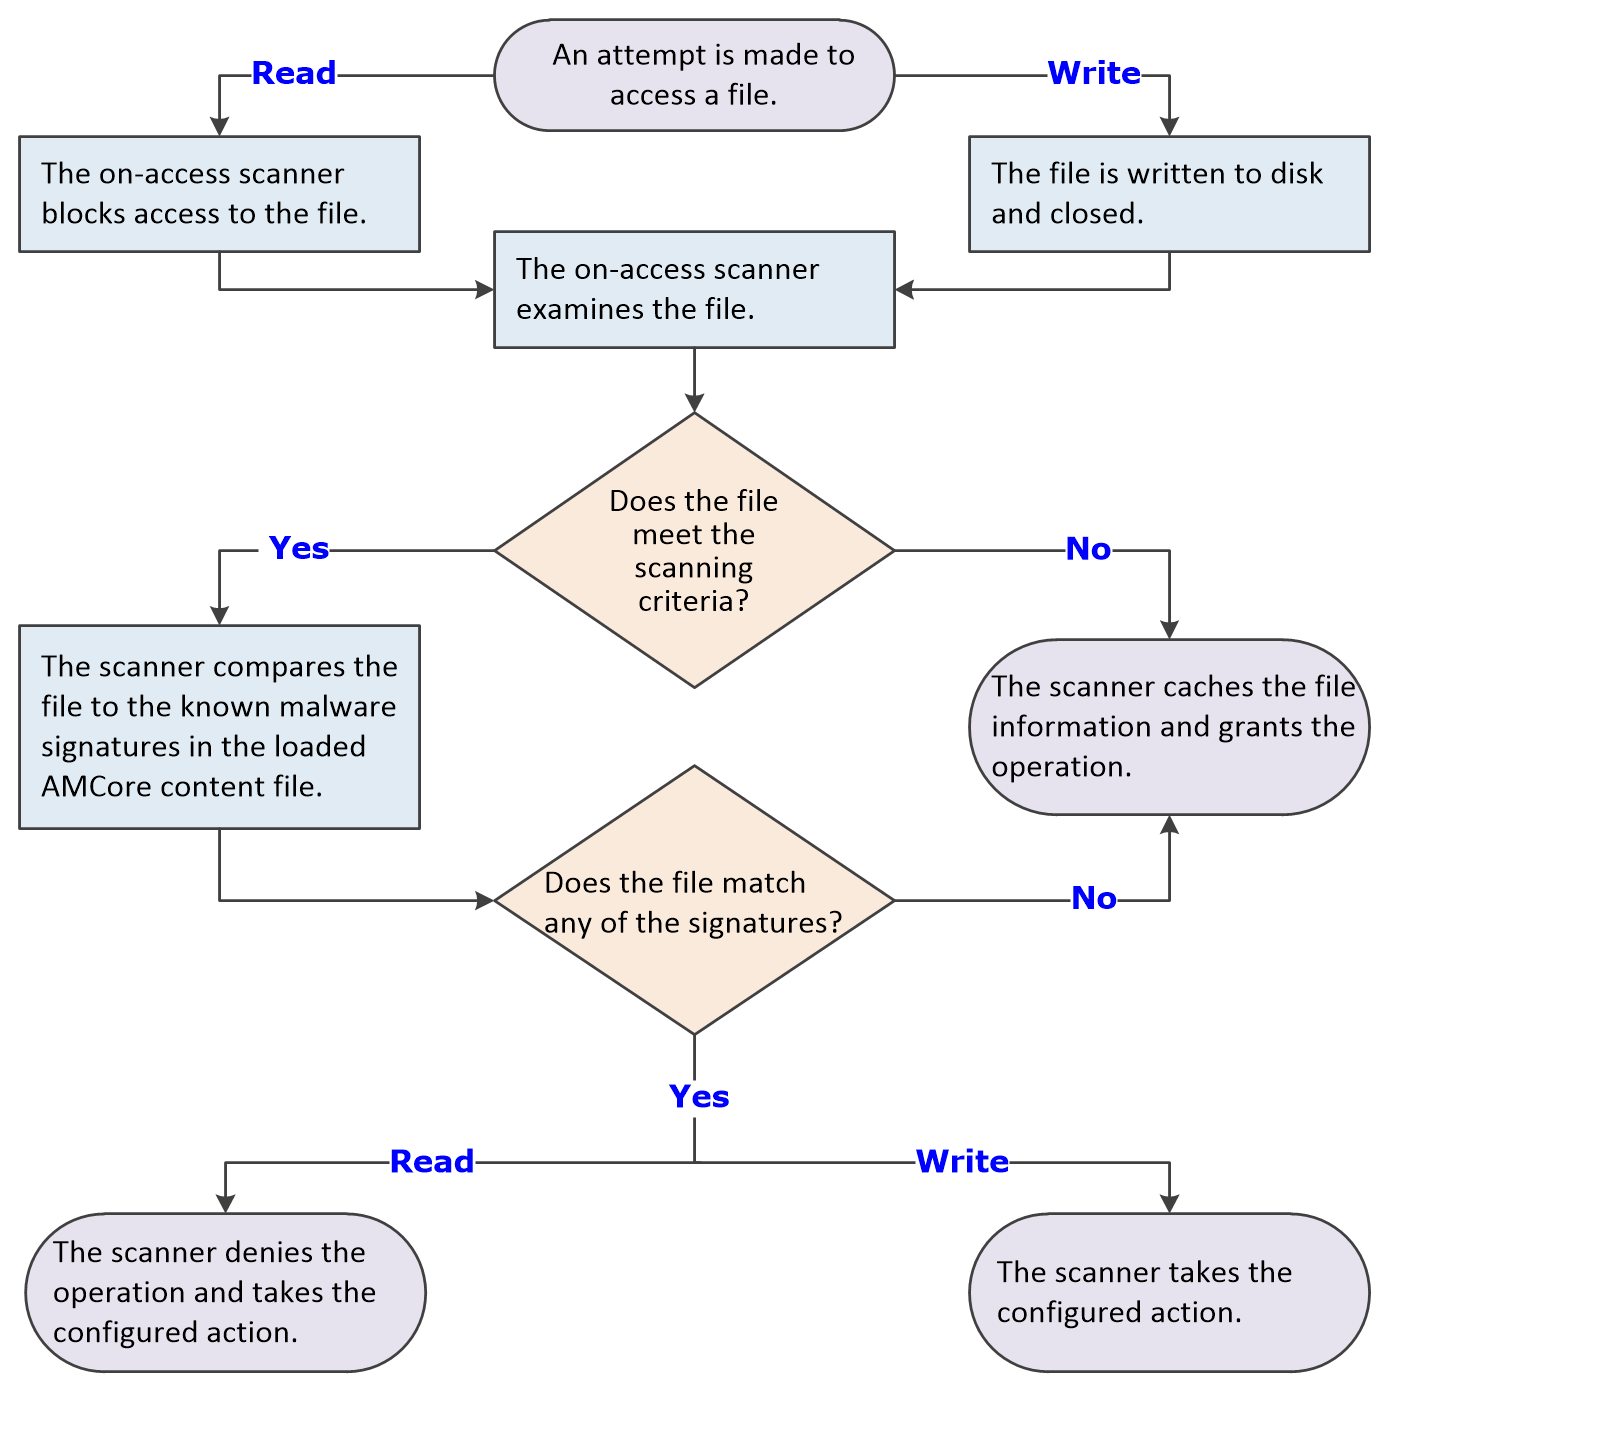
\includegraphics[scale=0.8]{images/onaccessscan.png}
\end{figure}

Because the scan depends on the pre-defined signature, a new malware could
bypass these rules if it uses a novel method to infect or hide. The rules can
be bypassed by applying obfuscation in the malware code, which hides traces of
evident behavior.

Scanning for signature using machine learning is still a new method, and even
though some vendors tried, the progress is not much positive. A security
researcher has created a sample malware bypassing the Cylance Smart Anti-Virus
in less than 15 minutes \cite{cylance}.
